\documentclass[handout]{beamer}
\usetheme[]{Szeged}
\usecolortheme{beaver}
\setbeamertemplate{footline}[frame number]
\usepackage[utf8]{inputenc}
\usepackage[spanish,es-nodecimaldot]{babel}
\usepackage{amsmath, amsthm, amsfonts, amssymb}
\usepackage{textcomp}
\usepackage{multimedia}
\DeclareGraphicsExtensions{.png,.pdf,.jpg,.jpeg}
\graphicspath{{imagenes/}} %directorio donde se guardan las imagenes
\usepackage{hyperref}
\usepackage{enumitem}

\SetLabelAlign{parright}{\parbox[t]{\labelwidth}{\raggedleft#1}}
\setlist[description]{style=multiline,topsep=10pt,leftmargin=4cm,align=parright}
\setlist[itemize]{label=\textbullet}

\title{Física II}
\author{Hidródinámica}
\institute[UVM]{4\textdegree \hspace{2pt} cuatrimestre.}
\logo{
\includegraphics[width=1.2cm]{uvm}}
\date{\today}

\begin{document}

\begin{frame}[noframenumbering]
  \titlepage
  \begin{center}
    
\includegraphics[width=5.5cm]{uvm1}    
  \end{center}  
\end{frame}


\begin{frame}
  \frametitle{Hidrodinámica}
  \begin{block}{Consideraciones sobre los líquidos}
    \begin{itemize}
    \item Los líquidos son incompresibles por completo.
    \item La viscosidad es despreciable.
    \item El flujo de los líquidos es estable.
    \end{itemize}
  \end{block}
\end{frame}

\begin{frame}[allowframebreaks,t]
  \frametitle{Gasto}
  
  {\huge \[G= \frac{V}{t}\]}
  
  \begin{tabular}{ll}
    $G:$ & Gasto (m$^3$/s).  \\ 
    $V:$ & Volumen del líquido que fluye (m$^3$). \\ 
    $t:$ & Tiempo en que tarda en fluir (s). \\
  \end{tabular}
  \begin{center}
    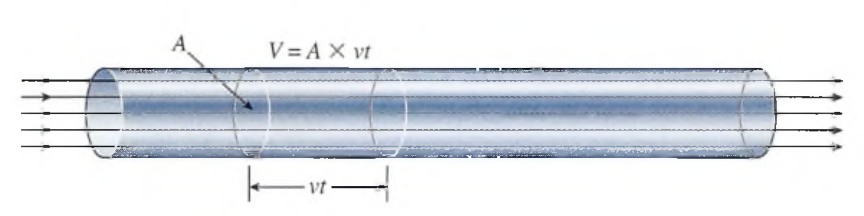
\includegraphics[width=10cm]{continuidad}
  \end{center}
  \[
  G = \frac{V}{t} = \frac{Avt}{t} = Av
  \]

  {\huge \[G = Av\]}

  \begin{tabular}{ll}
    $A:$ & Área de la sección tranversal (m$^2$).  \\ 
    $v:$ & Magnitud de la velocidad en la sección tranversal (m/s). \\
  \end{tabular}
  
\end{frame}


\begin{frame}[allowframebreaks,t]
  \frametitle{Ecuación de continuidad}
  \begin{block}{}
    La cantidad de líquido que pasa por un determinado tramo de tubería es la misma que
    pasa por otro tramo aunque sea más angosto. $G_{1} = G_{2}$
  \end{block}

  {\huge \[A_{1}v_{1} = A_{2}v_{2}\]}
  
  \begin{tabular}{ll}
    $A_{1}:$ & Área de la sección tranversal 1 (m$^2$).  \\ 
    $v_{1}:$ & Magnitud de la velocidad en la sección tranversal 1 (m/s). \\ 
    $A_{2}:$ & Área de la sección tranversal 2 (m$^2$).  \\ 
    $v_{2}:$ & Magnitud de la velocidad en la sección tranversal 2 (m/s). \\ 
  \end{tabular}
  \begin{center}
    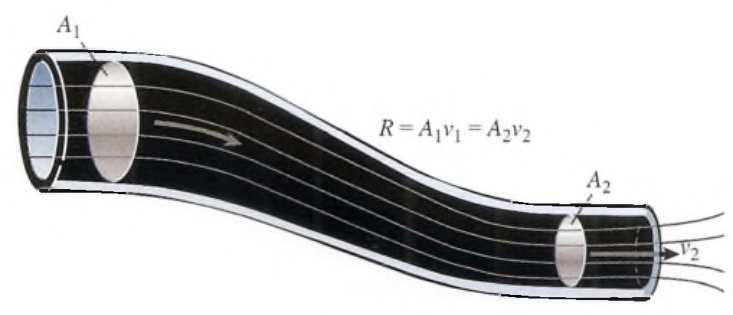
\includegraphics[scale=0.4]{continuidad2}
  \end{center}
\end{frame}


\begin{frame}
  \frametitle{Teorema de Bernoulli}
  \begin{block}{}
    En un líquido ideal cuyo flujo es estacionario, la suma de la energías cinética
    potencial y de presión que tiene el líquido en un punto es igual a la suma de estas
    energías en otro punto cualquiera.\\
  \end{block}
  \[
  E_{c_1} + E_{p_1} + E_{pr_1} =  E_{c_2} + E_{p_2} + E_{pr_2}
  \]
  \begin{center}
    {\huge \textbf{La energía se conserva}}
  \end{center}
\end{frame}


\section{Aplicaciones}

\subsection{Hidrostática}

\begin{frame}
  \frametitle{Barómetro de mercurio}
  \begin{center}
    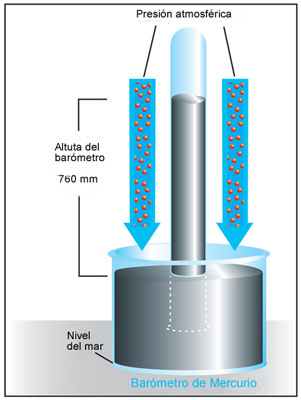
\includegraphics[width=5cm]{barometro}
  \end{center}
\end{frame}


\subsection{Hidrodinámica}

\begin{frame}
  \frametitle{Teorema de Torricelli}
  \begin{center}
    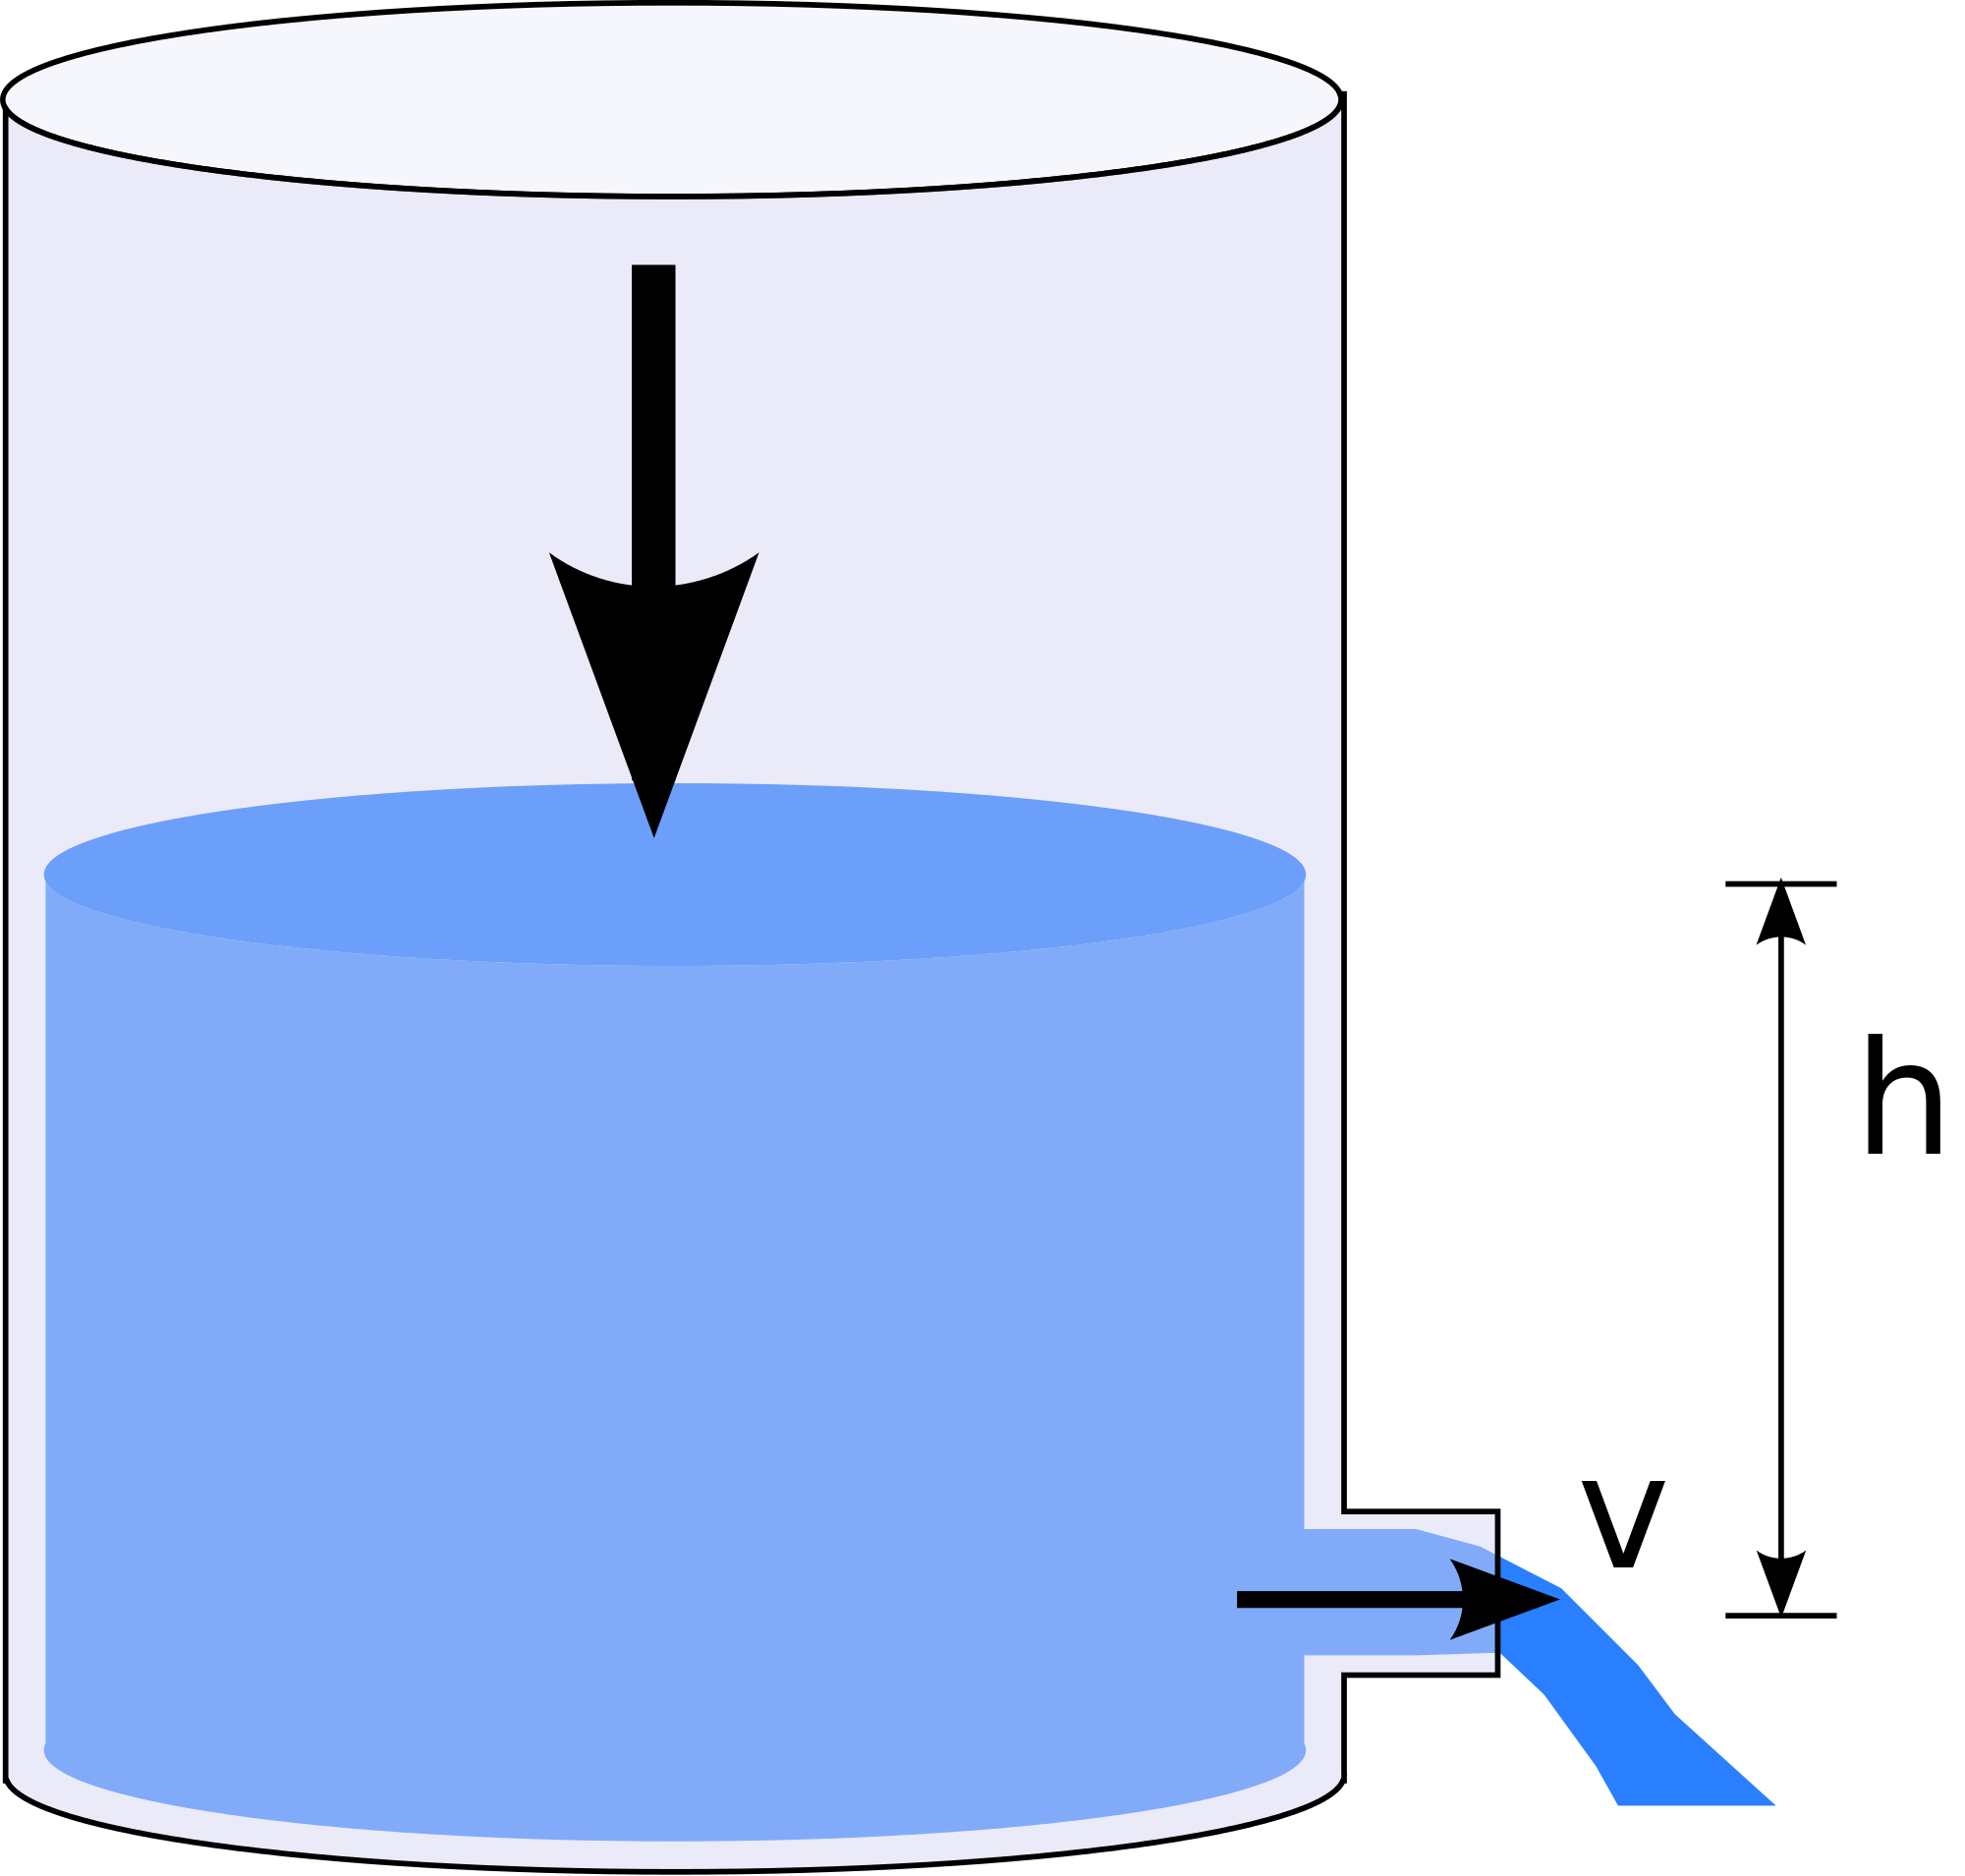
\includegraphics[width=5cm]{torricelli}
  \end{center}
\end{frame}


\begin{frame}
  \frametitle{Tubo de Pitot}
  % https://youtu.be/sYPIJ8Vz-FI?list=PLoh5n0Pf4HRRc9gSuF0ubX12sq2Z968bT
  \begin{center}
    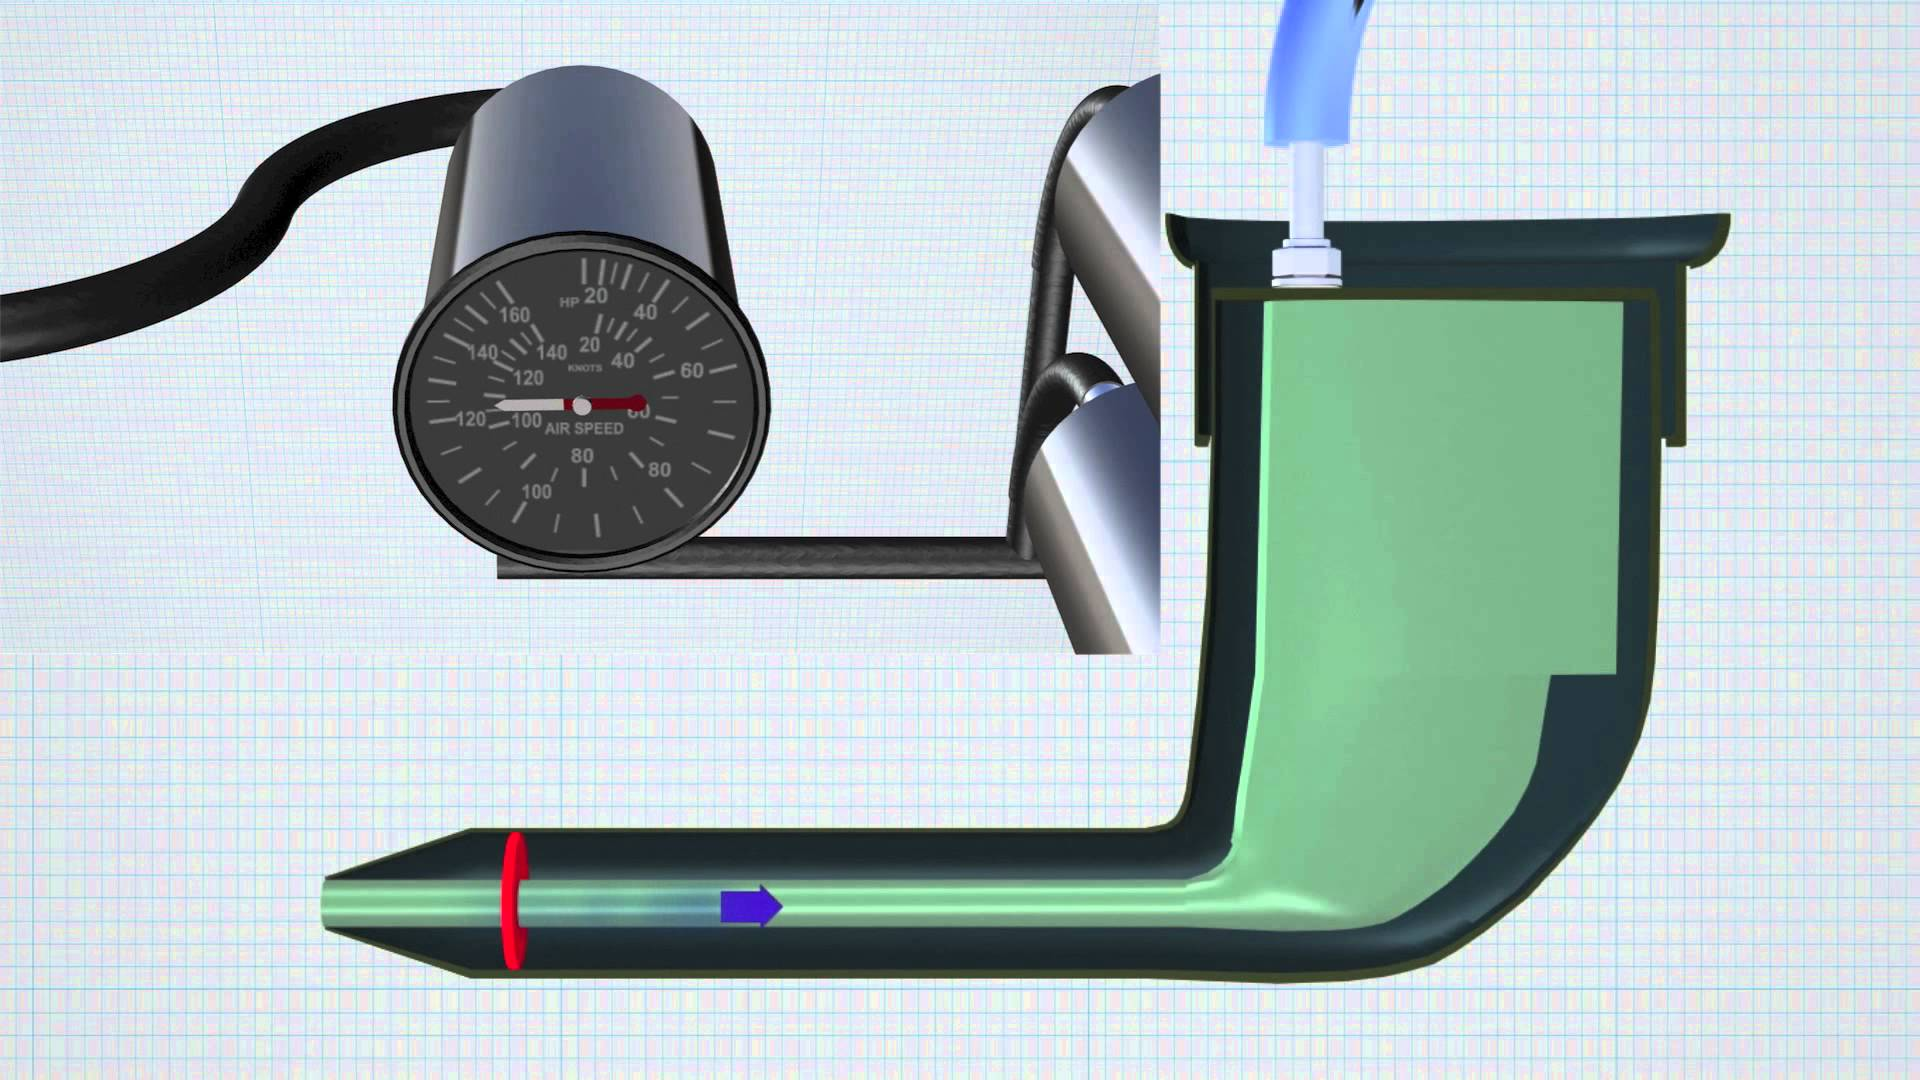
\includegraphics[width=7cm]{pitot}
  \end{center}
\end{frame}
% https://www.youtube.com/watch?v=mDDPiLkmbtg
% http://forum.lawebdefisica.com/threads/14590-Desaf%C3%ADo-2-07-El-bosque-inundado
\begin{frame}
  \frametitle{Tubo de Venturi}
  \begin{center}
    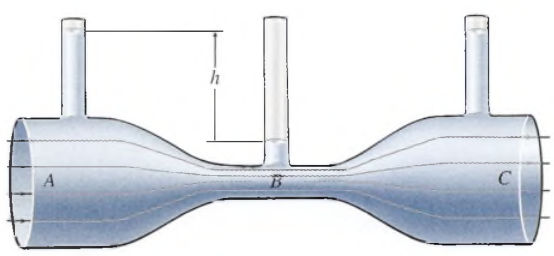
\includegraphics[width=8cm]{venturi}
  \end{center}
\end{frame}





\section{Ejercicios resueltos}

\begin{frame}[allowframebreaks,t]
\frametitle{Ejercicios resueltos}
\begin{enumerate}
\item Calcular el gasto en un tubería circular por la que circula
  petróleo si pasan 6 m$^3$ en 35 segundos.
\item Por una tubería de agua de sección transversal igual a 17 cm$^2$ la velocidad del
  agua es de 6 cm/s. Obtener el gasto de esa tubería.
\item En una manguera de 8 cm$^2$ circula agua a velocidad de 7 cm/s, si en la salida de
  la manguera el área se estrecha hasta tener un área de 2 cm $^2$, ¿cuál es la velocidad
  de salida en esa sección?
\item ¿Cuánto tiempo tardará en llenarse un Rotoplas (tanque de agua) de 1100 litros, si
  si se suministra un gasto de 0.02 m$^3$/s?
\item En una ferretería al comprar una manguera las especificaciones dicen que tiene un
  gasto promedio de 0.004 m$^3$/s. Si el diámetro de la manguera es de 4 cm, ¿cuál es la
  velocidad promedio que alcanza el líquido?
\item Calcular la velocidad de salida en la llave que se encuentra en el fondo de un
  tinaco si la altura que tiene el tinaco es de 2 m.
\end{enumerate}
\end{frame}


\begin{frame}
  \frametitle{Encuesta de evalución diagnóstica}
  \begin{center}
    
\includegraphics[scale=0.95]{qrevaluacion}
  \end{center}
\end{frame}

% https://encrypted.google.com/search?hl=en&q=videos%20de%20regimen%20turbulento


% \begin{frame}[allowframebreaks,t]
% \frametitle{Ejercicios propuestos}
% \begin{enumerate}
% \item holi
% \end{enumerate}
% \end{frame}


\end{document}